\documentclass[./../main.tex]{subfiles}
\graphicspath{{img/}}

\begin{document}
    \begin{exercise}
        A partir del modelo de la gota calcula las energías de enlace de los núcleos:

        \begin{solution}
            La expresión para la energía de ligadura que se obtiene a partir del modelo de la gota está dada como:

            \begin{equation}
                B.E.(A, Z) = a_{1}A - a_{2}A^{2/3} - a_{3}\dfrac{Z^{2}}{A^{1/3}} - a_{4}\dfrac{(N - Z)^{2}}{A} \pm a_{5}A^{-3/4},
                \label{eq:BindingEnergyLiquidDropModel} 
            \end{equation}

            donde el último término es positivo si el núcleo es par-par, negativo si es impar-impar o cero en cualquier otro caso.

            Notemos que podemos reescribir \cref{eq:BindingEnergyLiquidDropModel}, ya que se nos pide calcular la energía de enlace para núcleos isóbaros, \idest \(A = 76\). Así,

            \begin{align}
                B.E.(76, Z) &= 76a_{1} - 76^{2/3}a_{2} - \dfrac{Z^{2}}{76^{1/3}}a_{3} - \dfrac{(N - Z)^{2}}{76}a_{4} \pm 76^{-3/4}a_{5},\nonumber\\
                B.E.(76, Z) &= \left[\num{876.571} - \num{0.169979}Z^{2} - \num{0.306579}(N - Z)^{2} \pm \num{1.3209}\right]\unit{\MeV},\label{eq:ReducedBindingEnergy}
            \end{align}

            donde \(a_{1} \approx \qty{15.5}{\MeV}\), \(a_{2} \approx \qty{16.8}{\MeV}\), \(a_{3} \approx \qty{0.72}{\MeV}\), \(a_{4} \approx \qty{23.3}{\MeV}\) y \(a_{5} \approx \qty{34}{\MeV}\).

            \begin{table}[htb]
                \centering
                \begin{tblr}{
                    colspec = {cccc},
                    hlines,
                    vlines,
                    row{1} = {font = \bfseries},
                }
                    N          &    Z    & Elemento      &     Tipo     \\
                    45         &   31    &  \ch{Ga}      & impar-impar  \\
                    44         &   32    &  \ch{Ge}      & par-par      \\
                    43         &   33    &  \ch{As}      & impar-impar  \\
                    42         &   34    &  \ch{Se}      & par-par      \\
                    41         &   35    &  \ch{Br}      & impar-impar  \\
                    40         &   36    &  \ch{Kr}      & par-par      \\
                \end{tblr}
                \caption{Información de los núcleos con \(A = 76\): número de neutrones \(N\), número de protones \(Z\), elemento y si el núcleo es par-par o impar-impar.}
              \label{tblr:nucleusInformation}
            \end{table}

            \pagebreak
            Por un lado, para los núcleos par-par (\ch{^{76}Ge}, \ch{^{76}Se}, \ch{^{76}Kr} [\cref*{tblr:nucleusInformation}]) el último término de \cref{eq:ReducedBindingEnergy} es positivo.
            
            \begin{itemize}
                \item \ch{^{76}Ge}
                
                La energía de ligadura es de

                \begin{align*}
                    B.E.(76, 32) &= \left[\num{876.571} - \num{0.169979}(32)^{2} - \num{0.306579}(44 - 32)^{2} + \num{1.3209}\right]\unit{\MeV},\\
                    \Aboxedmain{B.E.(76, 32) &= \qty{659.686}{\MeV}.}
                \end{align*}
                
                \item \ch{^{76}Se}
                
                La energía de ligadura es de

                \begin{align*}
                    B.E.(76, 34) &= \left[\num{876.571} - \num{0.169979}(34)^{2} - \num{0.306579}(42 - 34)^{2} + \num{1.3209}\right]\unit{\MeV},\\
                    \Aboxedmain{B.E.(76, 34) &= \qty{661.775}{\MeV}.}
                \end{align*}
                
                \item \ch{^{76}Kr}
                
                La energía de ligadura es de

                \begin{align*}
                    B.E.(76, 36) &= \left[\num{876.571} - \num{0.169979}(36)^{2} - \num{0.306579}(40 - 36)^{2} + \num{1.3209}\right]\unit{\MeV},\\
                    \Aboxedmain{B.E.(76, 36) &= \qty{652.694}{\MeV}.}
                \end{align*}
            \end{itemize}

            Por el otro, para los núcleos impar-impar (\ch{^{76}Ga}, \ch{^{76}As}, \ch{^{76}Br} [\cref*{tblr:nucleusInformation}]) el último término de \cref{eq:ReducedBindingEnergy} es negativo.

            \begin{itemize}
                \item \ch{^{76}Ga}
                
                La energía de ligadura es de

                \begin{align*}
                    B.E.(76, 31) &= \left[\num{876.571} - \num{0.169979}(31)^{2} - \num{0.306579}(45 - 31)^{2} - \num{1.3209}\right]\unit{\MeV},\\
                    \Aboxedmain{B.E.(76, 31) &= \qty{651.811}{\MeV}.}
                \end{align*}
                
                \item \ch{^{76}As}
                
                La energía de ligadura es de

                \begin{align*}
                    B.E.(76, 33) &= \left[\num{876.571} - \num{0.169979}(33)^{2} - \num{0.306579}(43 - 33)^{2} - \num{1.3209}\right]\unit{\MeV},\\
                    \Aboxedmain{B.E.(76, 33) &= \qty{659.485}{\MeV}.}
                \end{align*}
                
                \item \ch{^{76}Br}
                
                La energía de ligadura es de

                \begin{align*}
                    B.E.(76, 35) &= \left[\num{876.571} - \num{0.169979}(35)^{2} - \num{0.306579}(41 - 35)^{2} - \num{1.3209}\right]\unit{\MeV},\\
                    \Aboxedmain{B.E.(76, 35) &= \qty{655.989}{\MeV}.}
                \end{align*}
            \end{itemize}
    
            (parece mucho, pero en realidad pueden ahorrarse muchos cálculos ¿sí lo ven?). Grafiquen los valores de estas energías de enlace (esto será útil para la siguiente tarea).

            Finalmente graficamos los resultados obtenidos.

            \begin{figure}[htb]
                \centering
                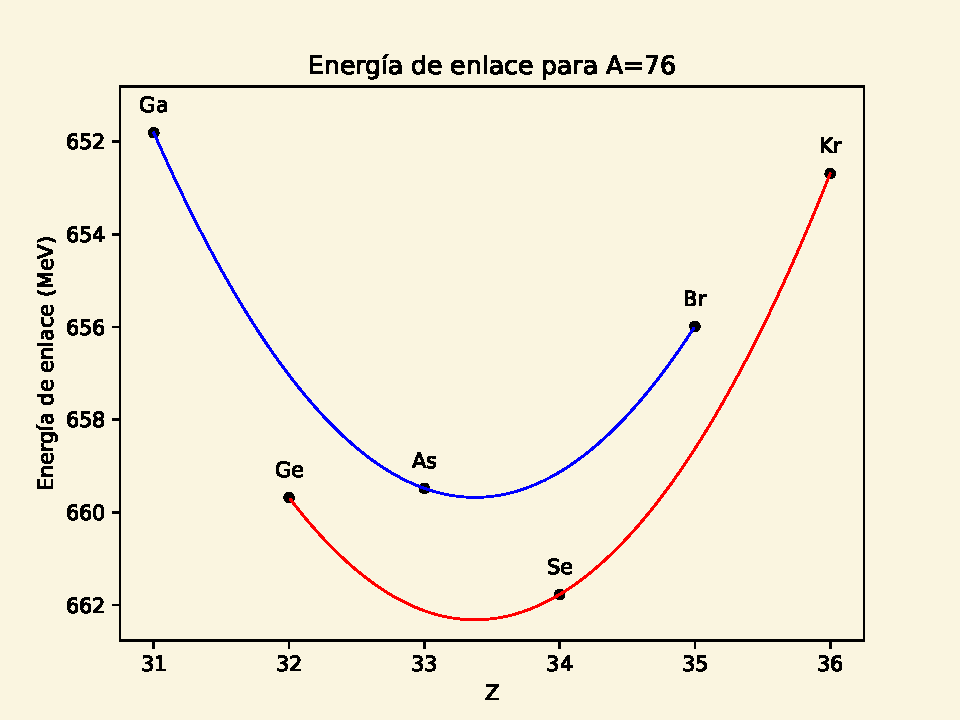
\includegraphics[scale=0.8]{binding_energy.pdf}
                \caption{Gráfica de las energías de ligadura vs. \(Z\) para los núcleos isóbaros de \(A = 76\).}
                \label{fig:}
            \end{figure}
        \end{solution}
    \end{exercise}
\end{document}